\chapter{流式主题模型的采样算法}
\label{chapter:sample}
Gibbs采样算法是LDA模型估计参数的一种主要方法。
但是朴素的Gibbs采样算法复杂度偏高,会随着LDA主题维度线性增长。
流式数据环境对算法的实时性要求很高。对于一批数据的处理,如果时间过长,有可能造成超时,数据堆积等等不稳定因素,
严重时会造成系统奔溃。
因而,本文采用了Metropolis-Hasting算法与Alias Table结合的方法将每次采样的复杂度降低到了$O(1)$。
不仅如此,本文还在此基础上进一步对采样算法的采样顺序进行了调整,使得采样过程中的网络使用率进一步得到了提升。

\section{Metropolis-Hastings采样}
统计采样是个很常见的问题,通常在进行采样之前,我们都需要知道采样的来自的具体分布。但是,也有很多时候采样的分布的概率形式非常复杂,或者很难计算得到。
因而通过计算概率分布之后再进行统计采样的的方法也会遇到困难。
MCMC(Markov Chain Monte Carlo, MCMC)方法是解决这种问题的常见途径。

\begin{theorem}[马氏链收敛定理]
如果一个非周期马氏链具有转移概率矩阵$P$, 且任何状态是连通的,那么有:

1. $\lim_{n\rightarrow \infty} P_{ij}^n = \pi(j)$

2. $\pi(j) = \sum_{i = 0}^{\infty}{\pi(i)P_{ij}}$

3. $\pi$是方程$\pi P = \pi$的唯一非负解

4. $\sum_{i=0}^{\infty}{\pi_i} =  1$

称分布$\pi$为马氏链的平稳分布。

\end{theorem}

从任何初始概率分布$\pi_0$出发,我们在马氏链上做状态转移,记$X_i$的概率分布为$\pi_i$,则有:
\begin{align*}
X_0 \sim \pi_0(x) \\
X_1 \sim \pi_1(x) \\
... \\
X_n \sim \pi_n(x) = \pi(x) \\
X_{n+1} \sim \pi(x) \\
X_{n+2} \sim \pi(x) \\
\end{align*}

由马氏链收敛定理,概率分布$\pi_i(x)$将收敛到平稳分布$\pi(x)$。假设到第$n$步的时候马氏链收敛,我们得到$X_n, X_{n+1}, X_{n+2}, ... \sim \pi(x)$是服从于同一个分布的随机变量。
那么如果从一个具体的初始状态$x_0$开始,沿着马氏链按照概率转移矩阵做跳转,
那么我们得到一个转移序列$x_0, x_1, x_2, ..., x_n , x_{n+1}, ...$,由于马氏链的收敛行为,我们知道$x_n, x_{n+1}, ...$都是来自于平稳分布$\pi(x)$的观测值。
使用这个绝妙的方法,我们便得到了一组来自于$\pi(x)$分布的样本。

根据上面的介绍,我们知道了在马氏链收敛定理中一个很关键的因素便是转移矩阵$P$,所以MCMC的一个关键问题便是如何定义和构造转移矩阵$P$,使得我们能够得到平稳的分布$\pi(x)$。

\begin{theorem}[细致平稳条件]
如果非周期马氏链的转移矩阵$P$和分布$\pi(x)$满足
\begin{equation}
\pi(i) P_{ij} = \pi(j) P_{ji}\mbox{  for all }i,j
\end{equation}
\end{theorem}

显然根据上面的细致平稳条件,我们很容易得出:
\begin{align*}
\sum_{i=1}^{\infty}{\pi(i) P_{ij}} = \sum_{i=1}^{\infty}{\pi(j) P_{ji}}= \pi(j) \Rightarrow \pi P = \pi
\end{align*}

给定非周期马氏链以及概率分布$p(x)$,现在假设已经得到了一个转移矩阵$Q$,用$q(i \rightarrow j)$表示从状态$i$转移到状态$j$的概率,
通常细致平稳条件并不成立:
\begin{align*}
p(i)q(i\rightarrow j) \neq p(j) q(j \rightarrow i)
\end{align*}

为了得到快速得到一个满足细致平稳条件的马氏链,我们对原来的马氏链做一些修改。
比如,引入接受概率$\alpha(i -> j)$使得
\begin{equation}
\label{eq:accept}
p(i) \underbrace{q(i \rightarrow j) \alpha(i \rightarrow j)}_{q^{\prime}(i \rightarrow j)}= p(j) \underbrace{q( j \rightarrow i ) \alpha(j \rightarrow i)}_{q^{\prime}(j \rightarrow i)}
\end{equation}
为了使得式\ref{eq:accept}成立,最简单的方式便是令
\begin{align*}
\alpha(i \rightarrow j ) = p(j)q(j \rightarrow i), \alpha(j \rightarrow i) = p(i) q(i \rightarrow j)
\end{align*}

通过上面改造,我们顺利得到了一个满足细致平稳条件的新的非周期马氏链,令其转移矩阵为$Q^{\prime}$。因此马氏链$Q^{\prime}$的平稳分布便是$p(x)$。
这个过程可以通俗地理解为在原来的马氏链$Q$上,从状态$i$以概率$q(i \rightarrow j)$转移到状态$j$需要通过接受概率$\alpha(i \rightarrow j)$。
因而,$q(i \rightarrow j)$也被称为提议分布。

尽管如此,我们发现目前接受概率被定义为两个概率的乘积,可想而知得到的接受概率$\alpha(i \rightarrow j)$会是一个比较小的小数,那么有很大的概率会转移失败。
如果失败太多次的话,会严重影响收敛到平稳分布的速度。

为此我们可以同比放大两边的接受概率而不破坏细致平稳条件,令:
\begin{equation}
\alpha(i \rightarrow j) = \min\left\{ \dfrac{p(j)q(j \rightarrow i)}{p(i)q(i \rightarrow j)},1 \right\}
\end{equation}

于是经过上面的改造,我们得到一个接受概率较大的又满足细致平稳条件的马氏链。
这种做法被称为Metropolis-Hastings采样算法\ref{alg:metropolis-hasting}
\begin{algorithm}[htb]  
\caption{Metropolis-Hastings Sampling} 
\label{alg:metropolis-hasting} 
\begin{algorithmic}[1] 
\State Set initial state of markov chain $X_0 = x_0$
\For{t = 0, 1, 2, ...}
\State Sample $y \sim q(x_t \rightarrow y)$
\State Sample $u \sim Uniform[0,1]$
\State Set $\alpha( x_t \rightarrow y) = \min \left\{ \dfrac{p(x_t)q(y \rightarrow x_t)}{p(y)q(x_t \rightarrow y)}, 1\right\}$
\If{$u < \alpha(x_t \rightarrow y)$}
\State Accept $x_t \rightarrow y$
\Else
\State Reject $x_t \rightarrow y$
\EndIf
\EndFor
\end{algorithmic}  
\end{algorithm}  

\section{Alias Table}

Alias Table\cite{vose1991a}是一项生成随机数的技术。给定一个概率分布$p(X)$,Alias Table能够按照概率分布$p(X)$以$O(1)$的时间复杂度生成一个随机数$x$。
不妨令$p(X) = \{p_0, p_1, ..., p_n\}$表示在变量$X=\{X_0, X_1, ..., X_n\}$上的分布,其中$\sum_i^n {p_i} = 1, p_i \ge 0$。
那么Alias Table技术等价于一次$O(n)$复杂度的初始化操作和任意次$O(1)$复杂的随机数生成操作。

算法\ref{alg:alias-table}中prob和alias是在Init步骤构建好的两个大小为$n$的表。

\begin{algorithm}[htb]  
\caption{Alias Table} 
\label{alg:alias-table}
\textbf{\underline{Rand:}}
\begin{algorithmic}[1] 
\State $u = Uniform(n)$
\State $j = \lfloor u \rfloor$
\If { $(u - j) \le \mbox{prob}[j]$ }
\Return $j$
\Else
~~\Return $\mbox{alias}[j]$
\EndIf
\end{algorithmic}  
\textbf{\underline{Init:}}
\begin{algorithmic}[1] 
\State l = 0; s = 0
\For{ $j = 0\mbox{ to } n - 1$}
\If{ $p_j > \frac{1}{n}$}
$\mbox{large}[l] = j; l = l + 1$
\Else
~~$\mbox{small}[s] = j; s = s + 1$
\EndIf
\EndFor
\While{ $s\ne 0\mbox{ and }l \ne 0$}
\State $s = s - 1; j = \mbox{small}[s]$
\State $l = l - 1; k = \mbox{large}[l]$
\State $\mbox{prob}[j] = n \times p_j$
\State $\mbox{alias}[j] = k$
\State $p_k = p_k + (p_j - \frac{1}{n})$
\If{ $p_k > \frac{1}{n}$}
$\mbox{large}[l] = k; l = l + 1$
\Else
~~$\mbox{small}[s] = k; s = s + 1$
\EndIf
\EndWhile
\While{ $s > 0$}
$s = s - 1; \mbox{prob}[\mbox{small}[s]] = 1$
\EndWhile
\While{ $l > 0$}
$l = l - 1; \mbox{prob}[\mbox{large}[l]] = 1$ \EndWhile
\end{algorithmic}  
\end{algorithm}  

Init算法实际上是对一个面积为1的区域进行填空的过程。
这种填空方法的思路主要来自于,如果把概率看做长度,变量的宽都为1,
对于均匀分布有所有变量的长度都为$\frac{1}{n}$,刚好组成一个面积为1的矩形区域。
相当于将面积1等分为$n$个区间,此时随机选取一个$(0, 1)$之间的值,便能立即确定其属于哪个区间。
但这只是特例,大多数时候有一部分变量的概率不到$\frac{1}{n}$,而另外一部分概率超过了$\frac{1}{n}$,
为了构造上面提到的矩形,Alias Table的算法采取优先填满每个等分区间(每个区间最多被两个随机数占用)的方式,用长板补短板,逐一填空。

\begin{figure}[htb]\centering
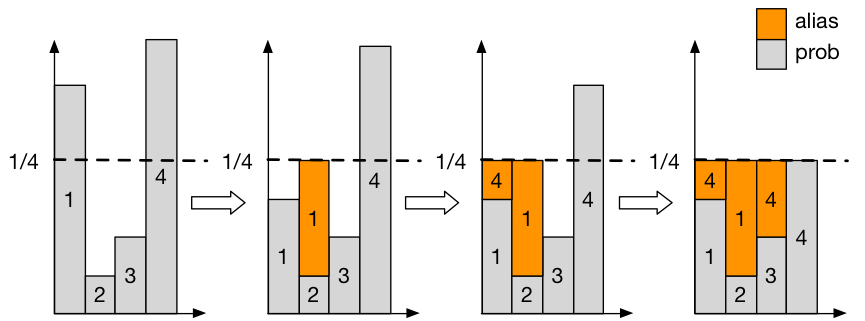
\includegraphics[width=0.8\linewidth]{alias-table}
\caption{Alias Table构建过程示意}
\label{fig:alias-table}       % Give a unique label
\end{figure}

如图\ref{fig:alias-table}, 实际上算法\ref{alg:alias-table}的Init步骤等价于在填写一个面积为1的矩形区域。

(1) 该矩形被等分为$n$份,每一份的面积等于$\frac{1}{n}$。

(2) 等分的$n$个子区域又各自分为prob和alias两部分,也就是$\mbox{len}(\mbox{prob}[i]) +\mbox{len}( \mbox{alias}[i]) = \frac{1}{n}$对于任意$i$都成立。

(3) 对于每个变量$X_i$,面积占比为$\mbox{area}[i] = \mbox{len}(\mbox{prob}[i]) + \sum_{j, alias[j]=i}{\mbox{len}(\mbox{alias[j]})}$。

(4) 对所有变量$X_i$,有$\mbox{area}[i] = p_i$。

\section{主题模型采样算法}
前面的章节已经简略地介绍了主题模型的Gibbs采样参数估计方法,Gibbs采样算法是Metropolis-Hastings算法接受概率为1的一个特例。
在LDA模型中我们会关心主题变量$z$在语料上的分布,然而我们事先并不知道$p\mathbf{ (z, w)}$的具体情况。
我们已经知道了通过MCMC方法可以收敛得到一些来自于某一稳定分布的样本。
为了应用MCMC来对LDA模型中的主题变量进行抽样,关键问题在于如何构建非周期性马氏链。
\begin{equation}
\label{eq:stable-cond}
p(z_i = x , \mathbf{z}_{\neg i}, \mathbf{w}) p( z_i = y | \mathbf{z}_{\neg i},  \mathbf{w})  =  
p(z_i = y , \mathbf{z}_{\neg i}, \mathbf{w}) p( z_i = x | \mathbf{z}_{\neg i},  \mathbf{w}) 
\end{equation}

根据公式\ref{eq:stable-cond},令$p( z_i = k | \mathbf{z}_{\neg i},  \mathbf{w})$为第$i$维的变量状态之间的转移概率,
那么在这个维度上各个状态之间的转换满足细致平稳条件。
现假设,LDA模型某一轮迭代的输入语料中有$M$个文档,文档的平均长度为$\bar{L}$,主题模型设定的主题变量个数为$K$。
那么Gibbs采样算法迭代一轮的时间复杂度为$O(M\times \bar{L} \times K)$,其中一次采样的复杂度为$O(K)$。
也就是说,随着主题模型变量个数的增大,模型的时间消耗随着线性增长。这种采样复杂度的效率较低,尤其在实时性要求高的环境中很难被应用。

\subsection{高效的提议分布}
实际上,造成Gibbs采样算法低效的主要原因是采样概率的计算比较复杂,并且需要被频繁地更新(每次采样之后都会得到更新)。
针对Gibbs采样算法效率低的问题,Sparse LDA利用了参数的稀疏性,将每次采样的算法复杂度降低到了$O(K_w)$。
Alias LDA算法同样利用了参数的稀疏性,但是引入了Metropolis-Hastings和Alias Table技术,将算法复杂度降低到了$O(K_d)$。
Light LDA同样应用了Metropolis-Hastings和Alias Table技术,将每次采样的算法复杂度降低到了$O(1)$,
但是这种方法需要交替地应用两种不同的提议分布,
以达到更好的收敛效果。
受到这些技术的启发,本文也提出了一种高效的采样算法。

我们发现,Metropolis-Hastings算法并不要求接受概率必须为1,并且对提议分布$Q$的定义也没有严格的要求。
提议分布$q(\cdot)$的选择对算法快速收敛到真实后验分布$p(\cdot)$具有重要的意义,
挑选得好的分布能够从两个方面提升采样效率:

(1) 从提议分布$q(\cdot)$中采样的效率要远远高于原分布$p(\cdot)$

(2) 非周期马氏链会迅速收敛到平稳状态

事实上,提议分布$q(\cdot)$的选择也是一个权衡利弊的过程。提议分布$q(\cdot)$和真实分布$p(\cdot)$越接近,则非周期马氏链收敛越快,
但是这么一来从$q(\cdot)$中采样可能和直接从$p(\cdot)$中抽样同样复杂。
反过来,如果选择一个不那么相似的提议分布$q(\cdot)$可以使得从$q(\cdot)$分布中采样效率非常高,但是马氏链收敛的速度可能会变极慢。

%本文中的采样算法采用了LightLDA中提及的Metropolis-Hastings方法。
%LightLDA拥有两个提议分布,并且交替地作为高效率的采样分布。

%在公式\ref{eq:sample-prob}中,第一项与文档主题计数$n_{k,d}$有关而与词汇主题计数$n_{k,w}$无关,
%另外一项则只和词汇主题计数$n_{k,w}$相关而与文档主题计数$n_{k,d}$无关。
%不难推理出,该采样公式中概率密度主要集中在那些词汇主题计数$n_{k,w}$和文档主题计数$n_{k,d}$都比较大的主题。
%因此,公式\ref{eq:sample-prob}两项均可以作为较好的主题采样分布的提议分布。

在公式\ref{eq:sample-prob}中,Gibbs采样分布与文档主题计数$n_{k,d}$和词汇主题计数$n_{k,w}$密切相关。
前面已经提到,造成Gibbs采样算法低效的一个重要原因是采样分布需要被频繁地更新。
然而,许多研究发现在短时间内主题的计数并不会发生巨大的改变。
尤其在流式数据环境下,本文提出的在线和增量流式主题模型方法中,受到主题分配词汇概率的Dirichlet先验,
每个时间片上的数据变动,对整体模型的影响进一步得到了约束。

本文提出的采样算法充分利用了上面提到的主题模型的特性。

\textbf{提议分布:}
\begin{equation}
 p_c(k) \propto p_w(k) p_d(k)
\end{equation}
其中:
\begin{equation}
\begin{aligned}
& p_w(z = k) \propto \dfrac{n_{k,w} +\eta}{n_{k, \cdot} + V \eta} \\
& p_d(z = k) \propto (n_{k,d} +\alpha) 
\end{aligned}
\end{equation}

\textbf{从状态$s$转移到$t$的接受率为:}
\begin{equation}
\begin{aligned}
& \alpha_c(z=k) = \min \left\{\dfrac{p(t) p_c(s)}{p(s)p_c(t)}, 1\right\} \\
& \dfrac{p(t) p_c(s)}{p(s)p_c(t)}= \dfrac{ (n_{t,d}^{\neg di} + \alpha)(n_{t,w}^{\neg di} + \eta) (n_{s,\cdot}^{\neg di} + V \eta) p_c(s)}
{ (n_{s,d}^{\neg di} + \alpha)(n_{s,w}^{\neg di} + \eta) (n_{t,\cdot}^{\neg di} + V \eta)p_c(t)}
\end{aligned}
\end{equation}

在上面的式子中,$n_{k,w}, n_{k, d}, n_{k, \cdot}$表示某一时刻主题模型参数中的相应值。
根据前面的分析假设,这些值在短时间内不会发生大的变化。
因而,分布$p_c(k)$与原采样分布$p(k)$比较相似,可以作为一个很好的提议分布。

本文设计的算法在每轮迭代中只会计算一次$p_w(k)$,对于每个文档只会计算一次$p_c(k)$。
然后执行预处理得到Alias Table,借助这项技术算法需要$O(K)$时间复杂度的预处理,但是每次采样只需要$O(1)$时间。
不仅如此,我们接受概率$\alpha_c(k)$的复杂度为$O(1)$,计算代价很低。
通过分析,不难发现算法执行一轮迭代的时间复杂度为$O(M \times \bar{L} + M \times K + W \times K)$,相比于原先的$O(M \times \bar{L} \times K)$。
不仅如此,我们发现$p_w(k)$和$p_d(k)$其实是两个高度稀疏的向量,借助这个特性,我们可以将采样的复杂度进一步降低到$O(M \times \bar{L} + M \times K_d + W \times K_w)$。


\subsection{优化算法采样顺序}

\begin{algorithm}[htb]
\caption{Sample in Natural Order}
\label{alg:natural-order}
\begin{algorithmic}[1] 
\Require TAB(V, Z), $\mathbf{k} = [1, 2, ..., K], \mathbf{w}$
\For { m = 1 to $M$ }
\For { n = 1 to $N_m$}
\State \textbf{Require} parameter $n(w_{mn}, \mathbf{k}) \sim$ TAB(V, Z)
\State SAMPLE($z_{mn}, n(w_{mn}, \mathbf{k})$)
\EndFor
\EndFor
\end{algorithmic}  
\end{algorithm}  
常见的主题模型Gibbs采样算法是坐标轴下降方法,交替轮换坐标轴逐一地采样更新。
在一般情形中,对语料采样通常是语料中词汇出现的自然顺序,先后地对出现的词汇执行采样,如算法\ref{alg:natural-order}。

\begin{algorithm}[htb]
\caption{Sample in Vocabulary Order} 
\label{alg:vocab-order}
\begin{algorithmic}[1]
\Require TAB(V, Z) = \textbf{\{Dense(V, Z), Sparse(V, Z)\}}, $\mathbf{k} = [1, 2, ..., K], \mathbf{w_d, w_s}$
\Function{DO\_SAMPLING}{$\mathbf{n(v_b, k), w}$}
\For { each $(m , n)$ where $w_{mn } \in \mathbf{v_b}$}
\State SAMPLE($z_{mn}, n(w_{mn}, \mathbf{k}), \mathbf{w}$)
\EndFor
\EndFunction
\For { each block $\mathbf{n(v_b, k)}$ in \textbf{Dense(V, Z)} }
\State Issue DO\_SAMPLING($\mathbf{n(v_b, k), w_d}$)
\EndFor
\State Set $\mathbf{v_s}$ as the low-frequent vocabulary local
\State Pull all $\mathbf{n(v_s, k)} \sim $ \textbf{Sparse(V, Z)}
\State Issue DO\_SAMPLING($\mathbf{n(v_s, k), w_s}$)
\end{algorithmic}  
\end{algorithm}  

根据LDA模型Gibbs采样的概率分布公式,词汇采样过程中将会使用到与词汇关联的词汇主题分布$n(w, \mathbf{k})$。
但是自然顺序,词汇在语料中的分布式散乱的,前后被采样的词汇基本上是不相同的,相当于每次采样都随机地访问了词汇-主题表TAB(V, Z)中的一行。

这种情况下词汇主题分布向量$n(w, \mathbf{k})$难以被复用(做到这点必须完全加载整张表,而前面分析提到这张表有可能超过单机内存的容量)。
另外一方面,如果不复用$n(w, \mathbf{k})$,则需要频繁地对参数服务器发起pull请求,这显然会增加网络请求的次数,
不仅产生了更多网络延迟同时也更容易造成参数服务器的响应瓶颈,更严重的情况可能造成参数服务器崩溃或者网络通信失败。
显然,这种访问效率是极其低效的。

实际上,Gibbs采样算法并没有严格要求采样的顺序。
根据主题模型参数数据结构的设计,令TAB(V, Z) = \{Dense(V, Z), Sparse(V, Z)\},
其中Dense(V, Z)表示稠密的参数矩阵,Sparse(V, Z)表示稀疏的<Key, Value>参数矩阵。

Dense(V, Z)所对应的词汇子集都是高频词,这些词汇在所有语料子集上都有很大的概率会出现。
根据这些特性,按块读取稠密矩阵Dense(V, Z),虽然有可能会下载一些无用的参数,但是将会大大提高网络传输的效率。

Sparse(V, Z)所对应的词汇子集含有大量的低频词,大部分词汇不大可能出现在所有的语料子集上。因而每个子集上的低频词词汇表只是全局低频词词汇表的一个较小的子集
。因为这部分参数高度稀疏,所以实际中可以完整下载本地所有需要的参数。

根据以上的参数数据结构特性,本文算法\ref{alg:vocab-order}实现中将文档分为高频词和低频词两部分。
之后对高频词部分按照词汇表顺序排序汇总。
同时对静态稠密的Dense(V, Z)参数矩阵进行分块。

当采样算法开始时,算法实现按照块读取的方式读取Dense(V, Z)参数稠密矩阵的一部分,并在语料文档中的稠密部分执行相应词汇的重采样。
执行完改步骤之后,从Sparse(V, Z)中pull将本地所有本地需要的低频词参数,并执行文档低频词部分的重采样。

\subsection{Pipeline参数更新}
当Gibbs采样是按照文本语料中词汇的自然顺序采样时,参数不得不等待所有语料中词汇都被采样之后在同步更新。
这种做法在采样过程中网络处于空闲状态,而在参数更新时又很容易出现网络使用高峰。

在按照上一小节的方式优化Gibbs采样顺序之后,我们发现每个词汇的主题分布向量无需互相等待,因而在一个词汇所有出现位置都经过采样之后便可以执行参数的增量更新。
这种方法称之为Pipeline,它将参数在时间维度上异步均摊地执行网络更新,不仅在采样过程中利用了网络,还有效地解决了网络高峰的问题。

\begin{figure}[htb]\centering
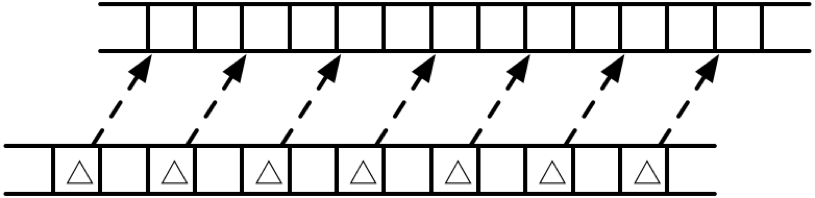
\includegraphics[width=0.7\linewidth]{pipeline}
\caption{Pipeline异步地进行网络传输}
\label{fig:pipeline}       % Give a unique label
\end{figure}


\begin{algorithm}[htb]
\caption{Pipeline Parameters Update} 
\label{alg:pipeline}
\begin{algorithmic}[1]
\Require TAB(V, Z) = \textbf{\{Dense(V, Z), Sparse(V, Z)\}}, $\mathbf{k} = [1, 2, ..., K], \mathbf{w_d, w_s}$
\Function{DO\_SAMPLING}{$\mathbf{n(v_b, k), w}$}
\For { each $(m , n)$ where $w_{mn } \in \mathbf{v_b}$}
\State GibbsSampling($z_{mn}, n(w_{mn}, \mathbf{k}), \mathbf{w}$)
\State Calculate update $\Delta \beta(w, \mathbf{k})$
\EndFor
\State Push $\Delta \beta(\mathbf{v_b}, \mathbf{k})$ to parameter
\EndFunction
\For { each block $\mathbf{n(v_b, k)}$ in \textbf{Dense(V, Z)} }
\State Issue DO\_SAMPLING($\mathbf{n(v_b, k), w_d}$)
\EndFor
\State Set $\mathbf{v_s}$ as the low-frequent vocabulary local
\State Pull all $\mathbf{n(v_s, k)} \sim $ \textbf{Sparse(V, Z)}
\State Issue DO\_SAMPLING($\mathbf{n(v_s, k), w_s}$)
\end{algorithmic}  
\end{algorithm}  

\section{实验分析}
\subsection{采样算法效率分析}

本节首先对本文提出的Metropolis-Hastings采样方法的效率进行实验设置。
\begin{figure}[htb]\centering
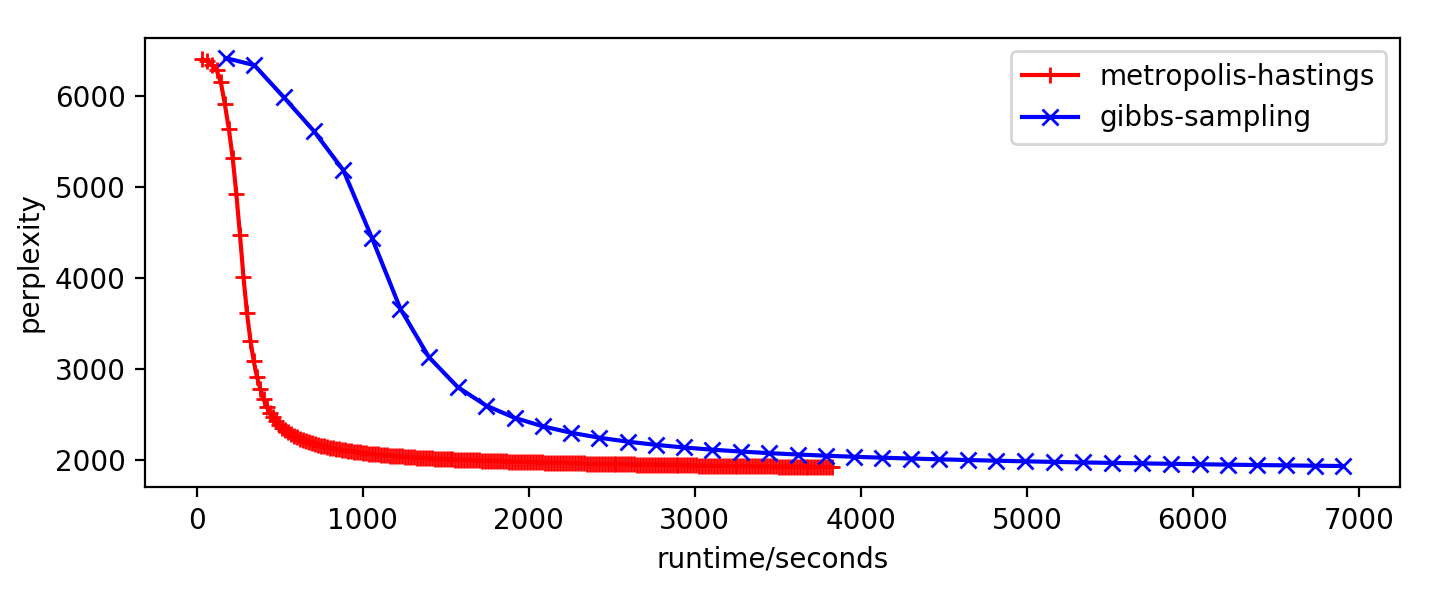
\includegraphics[width=1\linewidth]{exp-mh-vs-gibbs-perplexity-runtime}
\caption{本文Metropolis-Hastings方法与Gibbs采样算法效率对比}
\label{fig:mh-vs-gibbs}       % Give a unique label
\end{figure}

如图\ref{fig:mh-vs-gibbs},在实验中本文选取的Gibbs采样实现为GibbsLDA++\cite{gibbsLda++}。
为了更好地进行采样算法的效率对比,本文选取的主题模型训练法方式是在静态数据集上的批量学习方法。
在这个实验中,本文选取的语料中共有119301篇文档,53893799个词项;
主题模型的参数设置分别为$\alpha = 0.5, \eta = 0.01, K = 100$;
选取的评价指标为Perplexity。图中每个标记点均为一次迭代得到的Perplexity评估值。

通过对比,我们不难发现,Gibbs采样算法仅需要更少的迭代次数便能接近收敛,
但是本文提出的Metropolis-Hastings算法比Gibbs采样的收敛要更快。
这主要体现在Metropolis-Hastings算法采样的效率更高,迭代速度更快。
在实验过程中,我们发现Gibbs采样算法每轮迭代的平均时间消耗为180秒左右。
而本文的采样算法每轮迭代仅需要20秒。
事实上,如果我们将主题模型的主题个数$K$增大,这种差距会更加明显。

\subsection{算法网络效率分析}

本节实验主要从网络效率的角度分析本文采样算法的效率。
\begin{figure}[htb]\centering
\begin{subfigure}{1\textwidth}
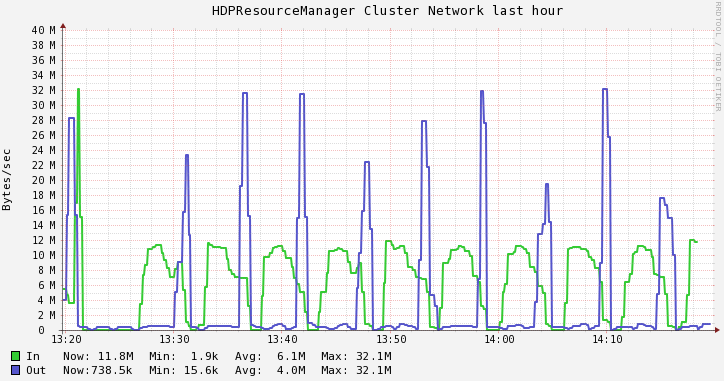
\includegraphics[width=0.75\linewidth]{exp-pipeline-hsq-network-1}
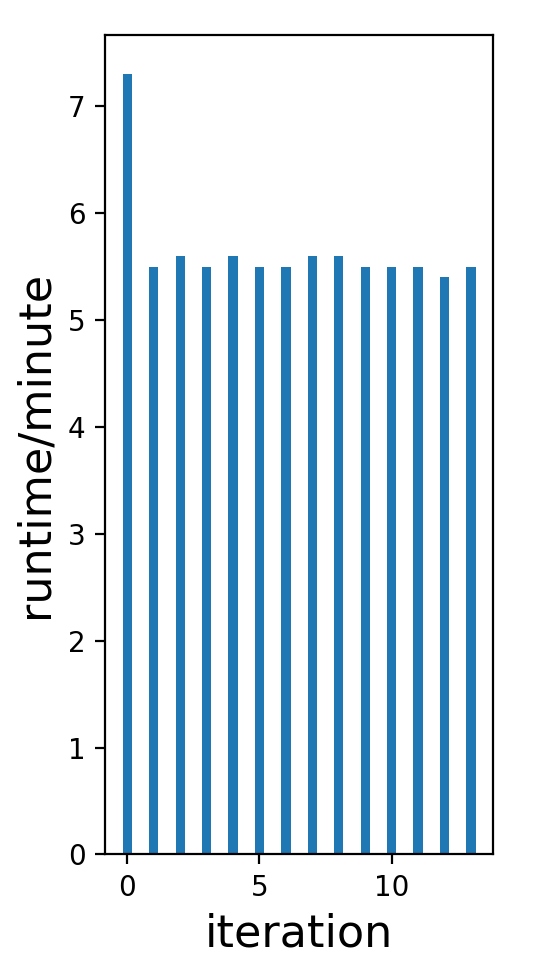
\includegraphics[width=0.23\linewidth]{exp-pipeline-hsq-runtime-1}
\caption{算法运行过程中未使用采样优化}
\end{subfigure}
\begin{subfigure}{1\textwidth}
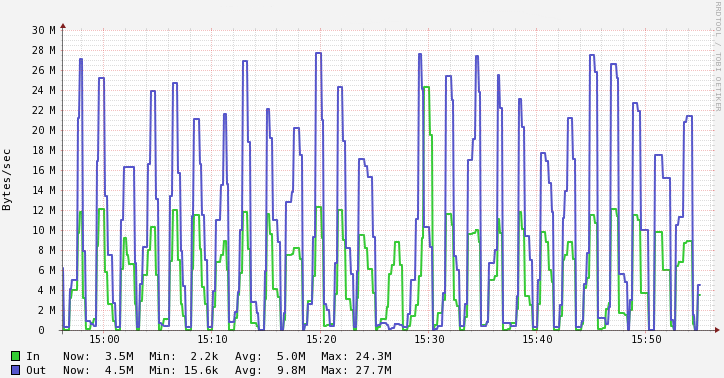
\includegraphics[width=0.75\linewidth]{exp-pipeline-hsq-network-2}
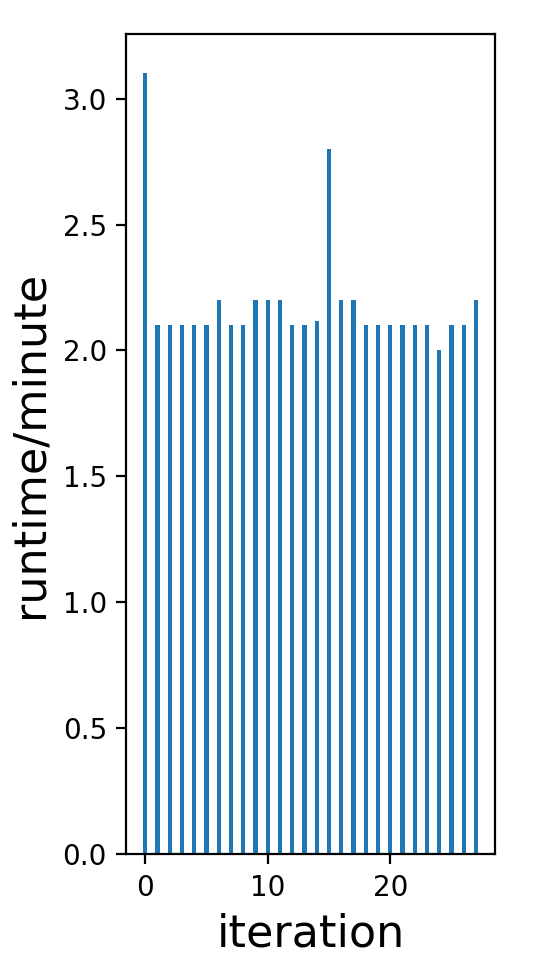
\includegraphics[width=0.23\linewidth]{exp-pipeline-hsq-runtime-2}
\caption{算法运行过程中使用了采样优化}
\end{subfigure}
\caption{采样算法的网络效率分析}
\label{fig:exp-pipeline}       % Give a unique label
\end{figure}

如图\ref{fig:exp-pipeline},在这两组实验中我们分别选择了是否进行采样优化,包括优化采样顺序和Pipeline更新。
两组实验中,左图为算法的网络流量图,右图为算法的迭代执行效率图。
网络流量图中,本文收集了算法迭代运行过程中的实时输入和输出网络流量,其中浅绿色峰值较小的是输入流量,深蓝色峰值较高的为输出流量。
造成输出流量波峰较高的原因主要是,输入流采样块读取机制,输出流采用随机索引更新的方式,造成了输出流的网络利用率更低。

通过对比两组实验,我们不难发现(a)组实验中输入流和输出流的的波峰明显是相互错开的,而(b)组实验中波峰是重叠在一起的。
事实上每个波峰对应着一次迭代,说明了(a)组实验的网络效率更低并且有巨大的延迟。
我们还发现,(b)组实验中几乎所有时刻网络都不存在空闲,平均网络的负载更大,但是网络峰值较低。
通过右图中的算法的执行迭代效率的对比也不难发现,两组实验的算法运行效率有着成倍的差异。
这个实验足以证明本文提出的采样算法优化不仅使得网络的利用更加充分、均衡,而且大幅提升了采样算法的效率和性能。

\section{本章小结}
Sparse LDA利用了主题模型参数的稀疏性来降低了采样的复杂度,
提出了一种Metropolis-Hastings和Alias Table相结合的新采样算法进一步提升了采样的效率。
这类加速技术对主题模型采样的效率具有非常大的意义,
因为原先朴素的采样方法的时间复杂度为$O(K)$,时间效率受到了主题变量维度大小的严重限制,
导致了许多时候无法使用高维的特征表达。

不仅如此,本文还提出了对算法采样顺序的优化以及Pipeline网络更新参数,大幅地提升了算法采样效率和性能。
在流式主题模型这种对时间效率要求极高的环境下,这种高效的采样方案为本文实时地进行大规模主题参数的采样的提供了可靠的保障。

